\documentclass[11pt,oneside]{article}	%use"amsart"insteadof"article"forAMSLaTeXformat
\usepackage{geometry}		%Seegeometry.pdftolearnthelayoutoptions.Therearelots.
\geometry{letterpaper}		%...ora4paperora5paperor...
%\geometry{landscape}		%Activateforforrotatedpagegeometry
%\usepackage[parfill]{parskip}		%Activatetobeginparagraphswithanemptylineratherthananindent
\usepackage{graphicx}				%Usepdf,png,jpg,orepswithpdflatex;useepsinDVImode
								%TeXwillautomaticallyconverteps-->pdfinpdflatex		
\usepackage{amssymb}
\usepackage{hyperref}

%----macros begin---------------------------------------------------------------
\usepackage{color}
\usepackage{amsthm}

\def\conv{\mbox{\textrm{conv}\,}}
\def\aff{\mbox{\textrm{aff}\,}}
\def\E{\mathbb{E}}
\def\R{\mathbb{R}}
\def\Z{\mathbb{Z}}
\def\tex{\TeX}
\def\latex{\LaTeX}
\def\v#1{{\bf #1}}
\def\p#1{{\bf #1}}
\def\T#1{{\bf #1}}

\def\vet#1{{\left(\begin{array}{cccccccccccccccccccc}#1\end{array}\right)}}
\def\mat#1{{\left(\begin{array}{cccccccccccccccccccc}#1\end{array}\right)}}

\def\lin{\mbox{\rm lin}\,}
\def\aff{\mbox{\rm aff}\,}
\def\pos{\mbox{\rm pos}\,}
\def\cone{\mbox{\rm cone}\,}
\def\conv{\mbox{\rm conv}\,}
\newcommand{\homog}[0]{\mbox{\rm homog}\,}
\newcommand{\relint}[0]{\mbox{\rm relint}\,}

%----macros end-----------------------------------------------------------------

\title{Curves, surfaces and splines with LAR
\footnote{This document is part of the \emph{Linear Algebraic Representation with CoChains} (LAR-CC) framework~\cite{cclar-proj:2013:00}. \today}
}
\author{Alberto Paoluzzi}
%\date{}							%Activatetodisplayagivendateornodate

\begin{document}
\maketitle
\nonstopmode

\begin{abstract}
In this module we implement above LAR most of the parametric methods for polynomial and rational curves, surfaces and splines discussed in the book~\cite{Paoluzzi2003a}, and implemented in the PLaSM language and in the python package pyplasm. 
\end{abstract}

\tableofcontents

%===============================================================================
\section{Introduction}
%===============================================================================



%===============================================================================
\section{Tensor product surfaces}
%===============================================================================

The tensor product form of surfaces will be primarily used, in the remainder of this module, to support the LAR implementation of polynomial (rational) surfaces. For this purpose, we start by defining some basic operators on function tensors.
In particular, a toolbox of basic tensor operations is given in Script 12.3.1. The ConstFunTensor operator produces a tensor of constant functions starting from a tensor of numbers; the recursive FlatTensor may be used to ?flatten? a tensor with any number of indices by producing a corresponding one index tensor; the InnerProd and TensorProd are used to compute the inner product and the tensor product of conforming tensors of functions, respectively.


\paragraph{Toolbox of tensor operations}

%-------------------------------------------------------------------------------
@D Multidimensional transfinite Bernstein-Bezier Basis
@{""" Toolbox of tensor operations """
def larBernsteinBasis (U):
	def BERNSTEIN0 (N):
		def BERNSTEIN1 (I):
			def map_fn(point):
				t = U(point)
				out = CHOOSE([N,I])*math.pow(1-t,N-I)*math.pow(t,I)
				return out
			return map_fn
		return [BERNSTEIN1(I) for I in range(0,N+1)]
	return BERNSTEIN0
@}
%-------------------------------------------------------------------------------

\subsection{Tensor product surface patch}

%-------------------------------------------------------------------------------
@D Tensor product surface patch
@{""" Tensor product surface patch """
def larTensorProdSurface (args):
	ubasis , vbasis = args
	def TENSORPRODSURFACE0 (controlpoints_fn):
		def map_fn(point):
			u,v=point
			U=[f([u]) for f in ubasis]
			V=[f([v]) for f in vbasis]
			controlpoints=[f(point) if callable(f) else f 
				for f in controlpoints_fn]
			target_dim = len(controlpoints[0][0])
			ret=[0 for x in range(target_dim)]
			for i in range(len(ubasis)):
				for j in range(len(vbasis)):
					for M in range(len(ret)):
						for M in range(target_dim): 
							ret[M] += U[i]*V[j] * controlpoints[i][j][M]
			return ret
		return map_fn
	return TENSORPRODSURFACE0
@}
%-------------------------------------------------------------------------------

\paragraph{Bilinear tensor product surface patch}

%-------------------------------------------------------------------------------
@D Bilinear surface patch
@{""" Bilinear tensor product surface patch """
def larBilinearSurface(controlpoints):
	basis = larBernsteinBasis(S1)(1)
	return larTensorProdSurface([basis,basis])(controlpoints)
@}
%-------------------------------------------------------------------------------

\paragraph{Biquadratic tensor product surface patch}

%-------------------------------------------------------------------------------
@D Biquadratic surface patch
@{""" Biquadratic tensor product surface patch """
def larBiquadraticSurface(controlpoints):
	basis1 = larBernsteinBasis(S1)(2)
	basis2 = larBernsteinBasis(S1)(2)
	return larTensorProdSurface([basis1,basis2])(controlpoints)
@}
%-------------------------------------------------------------------------------

\paragraph{Bicubic tensor product surface patch}

%-------------------------------------------------------------------------------
@D Bicubic surface patch
@{""" Bicubic tensor product surface patch """
def larBicubicSurface(controlpoints):
	basis1 = larBernsteinBasis(S1)(3)
	basis2 = larBernsteinBasis(S1)(3)
	return larTensorProdSurface([basis1,basis2])(controlpoints)
@}
%-------------------------------------------------------------------------------


%===============================================================================
\section{Transfinite B\'ezier}
%===============================================================================
%-------------------------------------------------------------------------------
@D Multidimensional transfinite B\'ezier
@{""" Multidimensional transfinite Bezier """
def larBezier(U):
	def BEZIER0(controldata_fn):
		N = len(controldata_fn)-1
		def map_fn(point):
			t = U(point)
			controldata = [fun(point) if callable(fun) else fun 
				for fun in controldata_fn]
			out = [0.0 for i in range(len(controldata[0]))]		
			for I in range(N+1):
				weight = CHOOSE([N,I])*math.pow(1-t,N-I)*math.pow(t,I)
				for K in range(len(out)):  out[K] += weight*(controldata[I][K])
			return out
		return map_fn
	return BEZIER0

def larBezierCurve(controlpoints):
	return larBezier(S1)(controlpoints)
@}
%-------------------------------------------------------------------------------

%===============================================================================
\section{Coons patches}
%===============================================================================

%-------------------------------------------------------------------------------
@D Transfinite Coons patches
@{""" Transfinite Coons patches """
def larCoonsPatch (args):
	su0_fn , su1_fn , s0v_fn , s1v_fn = args
	def map_fn(point):
		u,v=point
		su0 = su0_fn(point) if callable(su0_fn) else su0_fn
		su1 = su1_fn(point) if callable(su1_fn) else su1_fn
		s0v = s0v_fn(point) if callable(s0v_fn) else s0v_fn
		s1v = s1v_fn(point) if callable(s1v_fn) else s1v_fn
		ret=[0.0 for i in range(len(su0))]	
		for K in range(len(ret)):
			ret[K] = ((1-u)*s0v[K] + u*s1v[K]+(1-v)*su0[K] + v*su1[K] + 
			(1-u)*(1-v)*s0v[K] + (1-u)*v*s0v[K] + u*(1-v)*s1v[K] + u*v*s1v[K])
		return ret
	return map_fn
@}
%-------------------------------------------------------------------------------


%===============================================================================
\section{Bsplines}
%===============================================================================
The B-splines discussed in this section are called \emph{non-uniform}
because different spline segments may correspond to different
intervals in parameter space, unlike uniform B-splines. 
The basis polynomials, and consequently the spline shape and the other
properties, are defined by a non-decreasing sequence of real
numbers
\[
t_0 \leq t_1 \leq\cdots\leq t_n,
\]
called the {\it knot sequence}.  Splines of this kind are also named
\emph{NUB-splines} in the remainder of this book,\footnote{Some authors
call them non-uniform non-rational B-splines.  We prefer to emphasize
that they are polynomial splines.} where the name stands for
Non-Uniform B-splines. 

The knot sequence is used to define the basis polynomials which blend
the control points.  In particular, each subset of $k+2$ adjacent knot
values is used to compute a basis polynomial of degree $k$.  Notice
that some subsequent knots may coincide.  In this case we speak of 
\emph{multiplicity} of the knots.


\paragraph{Note}\index{Splines!number of points and joints}

In non-uniform B-splines the number $n+1$ of {\em knot values} is
greater than the number $m+1$ of control points $\p{p}_0, \ldots,
\p{p}_m$.  In particular, the relation
\begin{equation}
	n = m+k+1,
	\label{eq:knotsNumber}
\end{equation}
where $k$ is the \emph{degree} of spline segments, must hold between
the number of knots and the number of control points.  The quantity $h
= k+1$ is called the \emph{order} of the spline.  It will be useful
when giving recursive formulas to compute the B-basis polynomials. 
Let us remember, e.g., that a spline of order four is made of cubic
segments.


\paragraph{Non-uniform B-spline flexibility}
\index{Non-uniform B-splines!flexibility}

Such splines have a much greater flexibility than the uniform ones. 
The basis polynomial associated with each control point may vary
depending on the subset of knots it depends on.  Spline segments may
be parametrized over intervals of different size, and even reduced to
a single point.  Therefore, the continuity at a joint may be reduced, 
e.g.~from $C^{2}$ to $C^{1}$ to $C^{0}$ and even to none by suitably increasing the multiplicity
of a knot.

%-------------------------------------------------------------------------------
\subsection{Definitions}
%-------------------------------------------------------------------------------

\subsubsection{Geometric entities}

In order to fully understand the construction of a non-uniform B-spline, it may
be useful to recall the main inter-relationships among the 5 geometric
entities that enter the definition.

\paragraph{Control points} \hspace{-2mm}are denoted as $\p{p}_{i}$, 
with $0\leq i\leq m$.  A non-uniform B-spline usually approximates the control 
points. 

\paragraph{Knot values} \hspace{-2mm}are denoted as $t_{i}$, with $0\leq i\leq 
n$.  It must be $n = m+k+1$, where $k$ is the spline degree.
Knot values are used to define the B-spline polynomials. They also 
define the join points (or joints) between adjacent spline segments. 
When two consecutive knots coincide, the spline segment associated with 
their interval reduces to a point.

\paragraph{Spline degree} \hspace{-2mm}is defined as the degree of the
B-basis functions which are combined with the control points.  The
degree is denoted as $k$.  It is connected to the spline order $h =
k+1$.  The most used non-uniform B-splines are either cubic or quadratic.  The
image of a linear non-uniform B-spline is a polygonal line.  The image of a
non-uniform B-spline of degree $0$ coincides with the sequence of control
points.

\paragraph{B-basis polynomials} \hspace{-2mm}are denoted as $B_{i,h}(t)$.  They are
univariate polynomials in the $t$ indeterminate, computed by using the
recursive formulas of Cox and de Boor.  The $i$ index is associated with
the first one of values in the knot subsequence
$(t_{i},t_{i+1},\ldots,t_{i+h})$ used to compute $B_{i,h}(t)$.  The
second index is called \emph{order} of the polynomial.

\paragraph{Spline segments} \hspace{-2mm}are defined as polynomial vector functions
of a single parameter.  Such functions are denoted as $\p{Q}_{i}(t)$,
with $k\leq i\leq m$.  A $\p{Q}_{i}(t)$ spline segment is obtained by a
combination of the $i$-th control point and the $k$ previous points
with the basis polynomials of order $h$ associated to the same
indices.  It is easy to see that the number of spline segments is
$m-K+1$.


%-------------------------------------------------------------------------------
\subsection{Computation of a B-spline mapping}
%-------------------------------------------------------------------------------

The B-spline mapping, i.e. the vector-valued polynomial to be mapped over a 1D domain
discretisation by the \texttt{larMap} operator, is computed by making reference to the 
\texttt{pyplasm} implementation given by the \texttt{BSPLINE} contained in the 
\texttt{fenvs.py} library in the \texttt{pyplasm} package.

\texttt{BSPLINE} is a third-order function, that must be ordinately applied to 
\texttt{degree}, \texttt{knots}, and \texttt{controlpoints}.


%-------------------------------------------------------------------------------
\subsection{Domain computation}
%-------------------------------------------------------------------------------

%-------------------------------------------------------------------------------
@D Domain decomposition for 1D bspline maps
@{""" Domain decomposition for 1D bspline maps """
def larDom(knots,tics=32): 
	domain = knots[-1]-knots[0]
	return larIntervals([tics*domain])([domain])
@}
%-------------------------------------------------------------------------------

%-------------------------------------------------------------------------------
\subsection{Examples}
%-------------------------------------------------------------------------------

\paragraph{Two examples of B-spline curves using lar-cc}

%-------------------------------------------------------------------------------
@O test/py/splines/test08.py
@{""" Two examples of B-spline curves using lar-cc """
import sys
""" import modules from larcc/lib """
sys.path.insert(0, 'lib/py/')
from splines import *

controls = [[0,0],[-1,2],[1,4],[2,3],[1,1],[1,2],[2.5,1],[2.5,3],[4,4],[5,0]];
knots = [0,0,0,0,1,2,3,4,5,6,7,7,7,7]
bspline = BSPLINE(3)(knots)(controls)
obj = larMap(bspline)(larDom(knots))
VIEW(STRUCT( MKPOLS(obj) + [POLYLINE(controls)] ))

controls = [[0,1],[1,1],[2,0],[3,0],[4,0],[5,-1],[6,-1]]
knots = [0,0,0,1,2,3,4,5,5,5]
bspline = BSPLINE(2)(knots)(controls)
obj = larMap(bspline)(larDom(knots))
VIEW(STRUCT( MKPOLS(obj) + [POLYLINE(controls)] ))
@}
%-------------------------------------------------------------------------------


\paragraph{Bezier curve as a B-spline curve}

%-------------------------------------------------------------------------------
@O test/py/splines/test09.py
@{""" Bezier curve as a B-spline curve """
import sys
""" import modules from larcc/lib """
sys.path.insert(0, 'lib/py/')
from splines import *

controls = [[0,1],[0,0],[1,1],[1,0]]
bezier = larBezierCurve(controls)
dom = larIntervals([32])([1])
obj = larMap(bezier)(dom)
VIEW(STRUCT( MKPOLS(obj) + [POLYLINE(controls)] ))

knots = [0,0,0,0,1,1,1,1]
bspline = BSPLINE(3)(knots)(controls)
dom = larIntervals([100])([knots[-1]-knots[0]])
obj = larMap(bspline)(dom)
VIEW(STRUCT( MKPOLS(obj) + [POLYLINE(controls)] ))
@}
%-------------------------------------------------------------------------------


\paragraph{B-spline curve: effect of double or triple control points}


%-------------------------------------------------------------------------------
@O test/py/splines/test10.py
@{""" B-spline curve: effect of double or triple control points """
import sys
""" import modules from larcc/lib """
sys.path.insert(0, 'lib/py/')
from splines import *

controls1 = [[0,0],[2.5,5],[6,1],[9,3]]
controls2 = [[0,0],[2.5,5],[2.5,5],[6,1],[9,3]]
controls3 = [[0,0],[2.5,5],[2.5,5],[2.5,5],[6,1],[9,3]]
knots = [0,0,0,0,1,1,1,1]
bspline1 = larMap( BSPLINE(3)(knots)(controls1) )(larDom(knots))
knots = [0,0,0,0,1,2,2,2,2]
bspline2 = larMap( BSPLINE(3)(knots)(controls2) )(larDom(knots))
knots = [0,0,0,0,1,2,3,3,3,3]
bspline3 = larMap( BSPLINE(3)(knots)(controls3) )(larDom(knots))

VIEW(STRUCT( CAT(AA(MKPOLS)([bspline1,bspline2,bspline3])) + 
	[POLYLINE(controls1)]) )
@}
%-------------------------------------------------------------------------------


\paragraph{Periodic B-spline curve}

%-------------------------------------------------------------------------------
@O test/py/splines/test11.py
@{""" Periodic B-spline curve """
import sys
""" import modules from larcc/lib """
sys.path.insert(0, 'lib/py/')
from splines import *

controls = [[0,1],[0,0],[1,0],[1,1],[0,1]]
knots = [0,0,0,1,2,3,3,3]				# non-periodic B-spline
bspline = BSPLINE(2)(knots)(controls)
obj = larMap(bspline)(larDom(knots))  
VIEW(STRUCT( MKPOLS(obj) + [POLYLINE(controls)] ))

knots = [0,1,2,3,4,5,6,7]				# periodic B-spline
bspline = BSPLINE(2)(knots)(controls) 	
obj = larMap(bspline)(larDom(knots))
VIEW(STRUCT( MKPOLS(obj) + [POLYLINE(controls)] ))
@}
%-------------------------------------------------------------------------------

\paragraph{Effect of knot multiplicity on B-spline curve}


%-------------------------------------------------------------------------------
@O test/py/splines/test12.py
@{""" Effect of knot multiplicity on B-spline curve """
import sys
""" import modules from larcc/lib """
sys.path.insert(0, 'lib/py/')
from splines import *

points = [[0,0],[-1,2],[1,4],[2,3],[1,1],[1,2],[2.5,1]]
b1 = BSPLINE(2)([0,0,0,1,2,3,4,5,5,5])(points)
VIEW(STRUCT(MKPOLS( larMap(b1)(larDom([0,5])) ) + [POLYLINE(points)]))
b2 = BSPLINE(2)([0,0,0,1,1,2,3,4,4,4])(points)
VIEW(STRUCT(MKPOLS( larMap(b2)(larDom([0,5])) ) + [POLYLINE(points)]))
b3 = BSPLINE(2)([0,0,0,1,1,1,2,3,3,3])(points)
VIEW(STRUCT(MKPOLS( larMap(b3)(larDom([0,5])) ) + [POLYLINE(points)]))
b4 = BSPLINE(2)([0,0,0,1,1,1,1,2,2,2])(points)
VIEW(STRUCT(MKPOLS( larMap(b4)(larDom([0,5])) ) + [POLYLINE(points)]))
@}
%-------------------------------------------------------------------------------


TODO: extend biplane mapping to unconnected domain ... (remove BUG above)



%===============================================================================
\section{NURBS}
%===============================================================================


Rational non-uniform B-splines are normally denoted as NURB splines or
simply as NURBS. These splines are very important for both graphics
and CAD applications. In particular:


\begin{enumerate}

\item 
Rational curves and splines are invariant with respect to affine and
projective transformations.  Consequently, to transform or
project a NURBS it is sufficient to transform or project its
control points, leaving to the graphics hardware the task of sampling
or rasterizing the transformed curve.

\item 
NURBS represent exactly the conic sections, i.e.~circles, ellipses, 
parabol\ae, iperbol\ae. Such curves are very frequent in mechanical 
CAD, where several shapes and geometric constructions are based on 
such geometric primitives.

\item
Rational B-splines are very flexible, since (a) the available degrees
of freedom concern both degree, control points, knot values and
weights; (b) can be locally interpolant or approximant; (c) can
alternate spline segments with different degree; and (d)
different continuity at join points.

\item
They also allow for local variation of ``parametrization velocity", or
better, allow for modification of the norm of velocity vector along
the spline, defined as the derivative of the curve with respect to the
arc length.  For this purpose it is sufficient to properly modify the
knot sequence.  This fact allows easy modification of the sampling density
of spline points along segments with higher or lower curvature, while
maintaining the desired appearance of smoothness.

\end{enumerate}

As a consequence of their usefulness for applications, NURBS are
largely available when using geometric libraries or CAD kernels.

%-------------------------------------------------------------------------------
\subsection{Rational B-splines of arbitrary degree}
%-------------------------------------------------------------------------------

A rational B-spline segment $\v{R}_{i}(t)$ is defined as the
projection from the origin on the hyperplane $x_{d+1}=1$ of a
polynomial B-spline segment $\v{P}_{i}(u)$ in $\E^{d+1}$ homogeneous
space.  

Using the same approach adopted when discussing rational B\'ezier
curves, where $\p{q}_{i} = (w_{i}\p{p}_{i}, w_{i})\in\E^{d+1}$ are the
$m+1$ homogeneous control points, the equation of the rational
B-spline segment of degree $k$ with $n+1$ knots, may be therefore
written as
\begin{equation}
    \p{R}_i(t) = 
    \sum_{\ell=0}^k 
    w_{i-\ell}\,\p{p}_{i-\ell} 
    {B_{i-\ell,k+1}(t) \over w(t)}
 = 
    \sum_{\ell=0}^k 
    \p{p}_{i-\ell} 
    N_{i-\ell,k+1}(t)
    \label{eq:NUBgeneriche1}
\end{equation}
with $ k\leq i\leq m$,  $t\in [t_{i}, t_{i+1})$, and
\[
w(t) = \sum_{\ell=0}^k
w_{i-\ell} B_{i-\ell,k+1}(t),
\]
where $N_{i,h}(t)$ is the non-uniform rational
B-basis function of initial value $t_{i}$ and order $h$.
A global representation of the NURB spline can be given, due to the 
local support of the $N_{i,h}(t)$ functions, i.e.~to the fact that 
they are zero outside the interval $[t_{i},t_{i+h})$. So:
\[
\p{R}(t) =  \bigcup_{i=k}^{m} \p{R}_i(t) = 
\sum_{i=0}^{m}\p{p}_{i}\,N_{i,h}(t), \qquad t\in [t_{k},t_{m+1}).
\]

NURB splines can be computed as non-uniform B-splines by using homogeneous
control points, and finally by dividing the Cartesian coordinate
maps times the homogeneous one.  This approach will be used in
the NURBS implementation given later in this chapter.  A more
efficient and numerically stable variation of the Cox and de Boor
formula for the rational case is given by
Farin~\cite{Farin:88}, p.~196.


%-------------------------------------------------------------------------------
\subsection{Computation of a NURBS mapping}
%-------------------------------------------------------------------------------

The NURBS mapping, i.e. the vector-valued polynomial to be mapped over a 1D domain
discretisation by the \texttt{larMap} operator, is computed by making reference to the 
\texttt{pyplasm} implementation given by the \texttt{RATIONALBSPLINE} contained in the 
\texttt{fenvs.py} library in the \texttt{pyplasm} package.

\texttt{RATIONALBSPLINE} is a third-order function, that must be ordinately applied to 
\texttt{degree}, \texttt{knots}, and \texttt{controlpoints}.

%-------------------------------------------------------------------------------
@D NURBS mapping definition
@{""" Alias for the pyplasm definition (too long :o) """
NURBS = RATIONALBSPLINE
@}
%-------------------------------------------------------------------------------

%-------------------------------------------------------------------------------
\subsection{Examples}
%-------------------------------------------------------------------------------


\begin{figure}[htbp] %  figure placement: here, top, bottom, or page
   \centering
   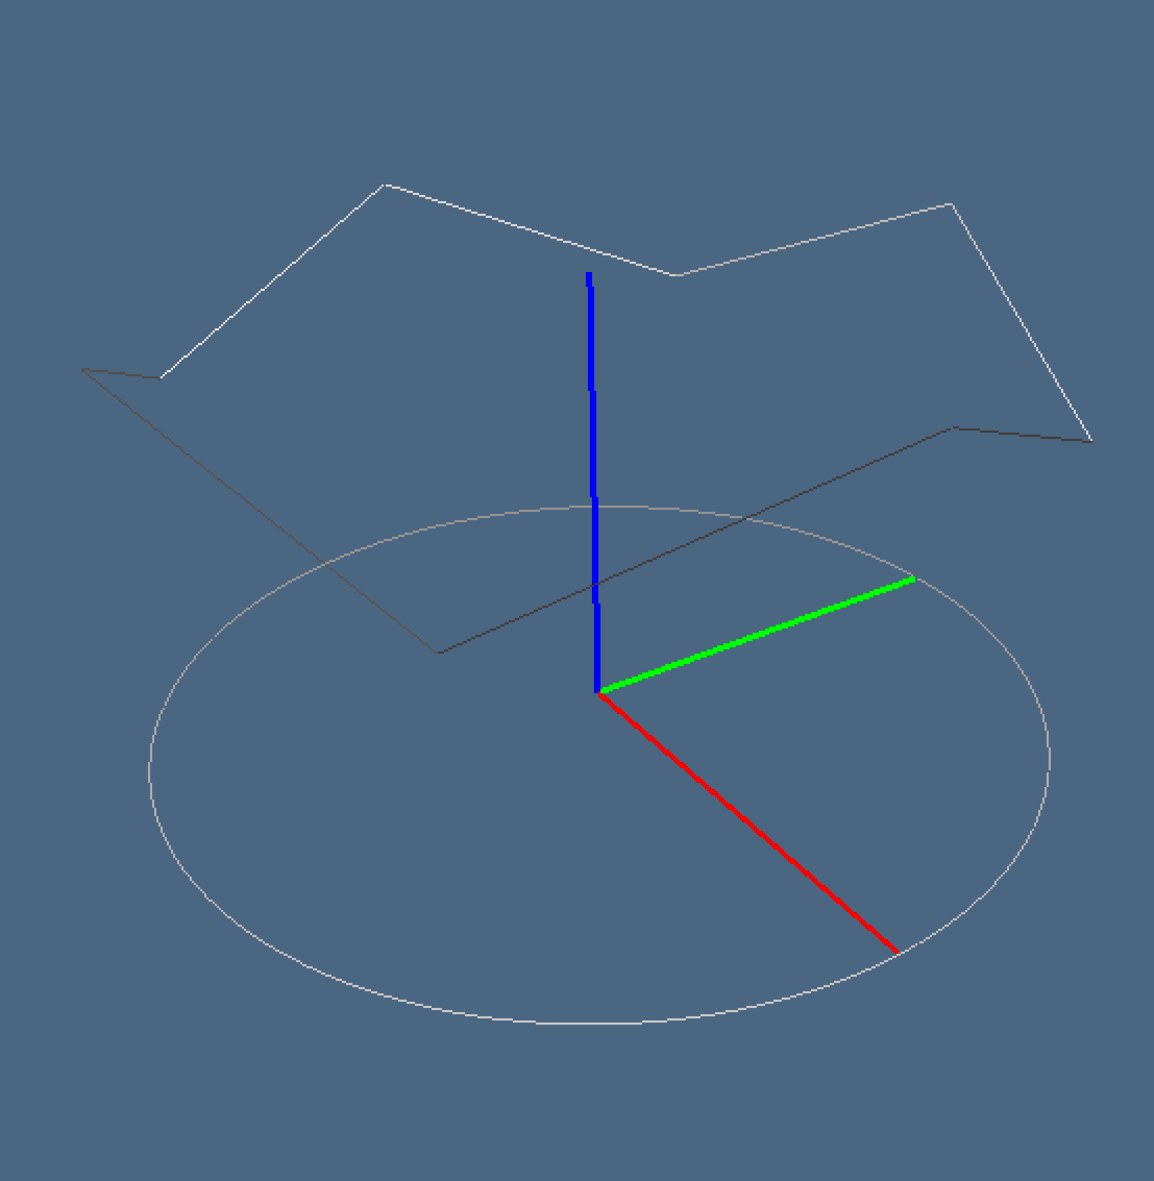
\includegraphics[width=0.33\linewidth]{images/nurbs-circle} 
   \caption{Circle 2D \emph{exactly} implemented as a 9-point NURBS curve.}
   \label{fig:example}
\end{figure}


\paragraph{Circle implemented as 9-point NURBS curve}

%-------------------------------------------------------------------------------
@O test/py/splines/test13.py
@{""" Circle implemented as 9-point NURBS curve """
import sys
""" import modules from larcc/lib """
sys.path.insert(0, 'lib/py/')
from splines import *

knots = [0,0,0,1,1,2,2,3,3,4,4,4]
_p=math.sqrt(2)/2.0
controls = [[-1,0,1], [-_p,_p,_p], [0,1,1], [_p,_p,_p],[1,0,1], [_p,-_p,_p], [0,-1,1], [-_p,-_p,_p], [-1,0,1]]
nurbs = NURBS(2)(knots)(controls)
obj = larMap(nurbs)(larDom(knots))
VIEW(STRUCT( MKPOLS(obj) + [POLYLINE(controls)] ))
@}
%-------------------------------------------------------------------------------



%===============================================================================
\section{Computational framework}
%===============================================================================
\subsection{Exporting the library}
%-------------------------------------------------------------------------------
@O lib/py/splines.py
@{""" Mapping functions and primitive objects """
@< Initial import of modules @>
@< Tensor product surface patch @>
@< Bilinear surface patch @>
@< Biquadratic surface patch @>
@< Bicubic surface patch @>
@< Multidimensional transfinite Bernstein-Bezier Basis @>
@< Multidimensional transfinite B\'ezier @>
@< Transfinite Coons patches @>
@< Domain decomposition for 1D bspline maps @>
@< NURBS mapping definition @>
@}


%===============================================================================
\section{Examples}
%===============================================================================

\paragraph{Examples of larBernsteinBasis generation}

%-------------------------------------------------------------------------------
@d Examples of larBernsteinBasis
@{larBernsteinBasis(S1)(3) 
""" [<function __main__.map_fn>,
	<function __main__.map_fn>,
	<function __main__.map_fn>,
	<function __main__.map_fn>] """
larBernsteinBasis(S1)(3)[0]
""" <function __main__.map_fn> """
larBernsteinBasis(S1)(3)[0]([0.0])
""" 1.0 """
@}
%-------------------------------------------------------------------------------

\paragraph{Graph of Bernstein-Bezier basis}

%-------------------------------------------------------------------------------
@O  test/py/splines/test04.py
@{""" Graph of Bernstein-Bezier basis """
import sys
""" import modules from larcc/lib """
sys.path.insert(0, 'lib/py/')
from splines import *

def larBezierBasisGraph(degree):
	basis = larBernsteinBasis(S1)(degree)
	dom = larDomain([32])
	graphs = CONS(AA(larMap)(DISTL([S1, basis])))(dom)
	return graphs

graphs = larBezierBasisGraph(4)
VIEW(STRUCT( CAT(AA(MKPOLS)( graphs )) ))
@}
%-------------------------------------------------------------------------------


\paragraph{Some examples of curves}

%-------------------------------------------------------------------------------
@O test/py/splines/test01.py 
@{""" Example of Bezier curve """
import sys
""" import modules from larcc/lib """
sys.path.insert(0, 'lib/py/')
from splines import *

controlpoints = [[-0,0],[1,0],[1,1],[2,1],[3,1]]
dom = larDomain([32])
obj = larMap(larBezierCurve(controlpoints))(dom)
VIEW(STRUCT(MKPOLS(obj)))

obj = larMap(larBezier(S1)(controlpoints))(dom)
VIEW(STRUCT(MKPOLS(obj)))
@}
%-------------------------------------------------------------------------------

\paragraph{Transfinite cubic surface}

%-------------------------------------------------------------------------------
@O test/py/splines/test02.py  
@{""" Example of transfinite surface """
import sys
""" import modules from larcc/lib """
sys.path.insert(0, 'lib/py/')
from splines import *

dom = larDomain([20],'simplex')
C0 = larBezier(S1)([[0,0,0],[10,0,0]])
C1 = larBezier(S1)([[0,2,0],[8,3,0],[9,2,0]])
C2 = larBezier(S1)([[0,4,1],[7,5,-1],[8,5,1],[12,4,0]])
C3 = larBezier(S1)([[0,6,0],[9,6,3],[10,6,-1]])
dom2D = larExtrude1(dom,20*[1./20])
obj = larMap(larBezier(S2)([C0,C1,C2,C3]))(dom2D)
VIEW(STRUCT(MKPOLS(obj)))
@}
%-------------------------------------------------------------------------------

\paragraph{Coons patch interpolating 4 boundary curves}

%-------------------------------------------------------------------------------
@O test/py/splines/test03.py  
@{""" Example of transfinite Coons surface """
import sys
""" import modules from larcc/lib """
sys.path.insert(0, 'lib/py/')
from splines import *
Su0 = larBezier(S1)([[0,0,0],[10,0,0]])
Su1 = larBezier(S1)([[0,10,0],[2.5,10,3],[5,10,-3],[7.5,10,3],[10,10,0]])
Sv0 = larBezier(S2)([[0,0,0],[0,0,3],[0,10,3],[0,10,0]])
Sv1 = larBezier(S2)([[10,0,0],[10,5,3],[10,10,0]])
dom = larDomain([20])
dom2D = larExtrude1(dom, 20*[1./20])
out = larMap(larCoonsPatch([Su0,Su1,Sv0,Sv1]))(dom2D)
VIEW(STRUCT(MKPOLS(out)))
@}
%-------------------------------------------------------------------------------


\paragraph{Bilinear tensor product patch}


%-------------------------------------------------------------------------------
@O test/py/splines/test05.py
@{""" Example of bilinear tensor product surface patch """
import sys
""" import modules from larcc/lib """
sys.path.insert(0, 'lib/py/')
from splines import *

controlpoints = [
	[[0,0,0],[2,-4,2]],
	[[0,3,1],[4,0,0]]]
dom = larDomain([20])
dom2D = larExtrude1(dom, 20*[1./20])
mapping = larBilinearSurface(controlpoints)
patch = larMap(mapping)(dom2D)
VIEW(STRUCT(MKPOLS(patch)))
@}
%-------------------------------------------------------------------------------

\paragraph{Biquadratic tensor product patch}

%-------------------------------------------------------------------------------
@O test/py/splines/test06.py
@{""" Example of bilinear tensor product surface patch """
import sys
""" import modules from larcc/lib """
sys.path.insert(0, 'lib/py/')
from splines import *

controlpoints=[
	[[0,0,0],[2,0,1],[3,1,1]],
	[[1,3,-1],[2,2,0],[3,2,0]],
	[[-2,4,0],[2,5,1],[1,3,2]]]
dom = larDomain([20])
dom2D = larExtrude1(dom, 20*[1./20])
mapping = larBiquadraticSurface(controlpoints)
patch = larMap(mapping)(dom2D)
VIEW(STRUCT(MKPOLS(patch)))
@}
%-------------------------------------------------------------------------------


\paragraph{Bicubic tensor product patch}

%-------------------------------------------------------------------------------
@O test/py/splines/test07.py
@{""" Example of bilinear tensor product surface patch """
import sys
""" import modules from larcc/lib """
sys.path.insert(0, 'lib/py/')
from splines import *

controlpoints=[
	[[ 0,0,0],[0 ,3  ,4],[0,6,3],[0,10,0]],
	[[ 3,0,2],[2 ,2.5,5],[3,6,5],[4,8,2]],
	[[ 6,0,2],[8 ,3 , 5],[7,6,4.5],[6,10,2.5]],
	[[10,0,0],[11,3  ,4],[11,6,3],[10,9,0]]]
dom = larDomain([20])
dom2D = larExtrude1(dom, 20*[1./20])
mapping = larBicubicSurface(controlpoints)
patch = larMap(mapping)(dom2D)
VIEW(STRUCT(MKPOLS(patch)))
@}
%-------------------------------------------------------------------------------



%===============================================================================
\appendix
\section{Utility functions}
%===============================================================================

\paragraph{Initial import of modules}

%-------------------------------------------------------------------------------
@D Initial import of modules
@{from pyplasm import *
from scipy import *
import os,sys
""" import modules from larcc/lib """
sys.path.insert(0, 'lib/py/')
from lar2psm import *
from simplexn import *
from larcc import *
from largrid import *
from mapper import *
@}
%-------------------------------------------------------------------------------


\bibliographystyle{amsalpha}
\bibliography{splines}

\end{document}
